\chapter{Crossdating and chronology building}
\label{txt:crossdating}
\index{Crossdating|(}

All algorithms work in pretty much the same way. There's a ``fixed'' sample, and there's a ``moving'' sample. Imagine you have printouts of their graphs on translucent paper. The fixed graph is taped to a table, and you can slide the moving sample left and right. This is actually how it was originally done, on graph paper, with one inch per decade. Start with the moving sample to the left of the fixed sample, overlapping it by 10 years. Look at how well the graphs match: this is the first score that's computed. Slide the moving sample to the right one year and so on until you reach the end.

You could do it all simply by moving graphs and eyeballing the crossdates like this but there are hundreds of sites and millennia of chronologies you'll want to crossdate your samples against, so that would take a while. Tellervo has a few algorithms to find likely crossdates almost instantaneously. They aren't perfect, though, and all crossdates should be inspected visually to ensure they are a good fit. 

\section{Algorithms}
Tellervo includes a total of five different algorithms for crossdating:


\subsection{T-Score}
\index{Crossdating!T-Score}
\index{T-Score}
The \textit{t}-score is the classic crossdate. Unfortunately, every dendro program seems to have a slightly different implementation of \textit{t}-score, so the numbers you get from Tellervo might not be exactly comparable to the numbers from other programs. 

The version Tellervo uses is based on the algorithms given in \citet{Baillie73}, though with some apparent bugs corrected (Ken Harris pers. comm.). In the following equations, $x_{0}, x_{1}, x_{2}, \dots$ are the data of the fixed sample in the overlap, $y_{0}, y_{1}, y_{2}, \dots$ are the data of the moving sample in the overlap, and N is the length of the overlap.

The first step is to make each dataset bivariate normal by replacing each value with the mean of the values around it, and then taking its natural logarithm.  The preparation for the \textit{t}-score is therefore done as follows and is done to both the fixed and moving series:

\begin{itemize}
 \item $x_{i} \leftarrow {x_{i-2} + x_{i} + x_{i+1} + x_{i+2} \over 5}$
 \item $x_{i} \leftarrow ln(_{xi})$
\end{itemize}

The student's T computation is then done as follows:

\begin{itemize}
 \item $s_{xy} = \Sigma x_{i} y_{i} - N (x_{i} - x_{avg}) (y_{i} - y_{avg})$
 \item $s_{xx} = \Sigma x_{i}^{2} - N (x_{i} - x_{avg})^{2}$
 \item $s_{yy} = \Sigma y_{i}^{2} - N (y_{i} - y_{avg})^{2}$
 \item $r = {s_{xy} \over \sqrt{(s_{xx} s_{yy})}}$
 \item $t = r \sqrt{{N-2\over 1-r^{2}}}$
\end{itemize}

The \textit{t}-score is an explorative statistic.  There is no univerally accepted threshold above which a \textit{t}-score is regarded as  significant, however, \citet{Baillie73} suggest a value of 3.5.  For more information see \citet{wigley1987}.


\subsection{Trend}
\index{Crossdating!Trend}
\index{Trend}
Trend is another popular crossdate statistic.  It computes the percentage of years with the same trend (going-up- or going-down-ness). Scores greater than 60\%-70\% are good. Trend is also referred to as ufigkeitsko-Gleichläeffizient, Gleichläufigkeit and Eckstein's W.

The trend is the simplest crossdate. For each sample, it computes the trend of each 2-year interval (1001-1002, 1002-1003, and so on). The trend of a 2-year interval is simply whether the next ring is larger, smaller, or the same. The trend score is the percentage of intervals in the overlap which are the same. For example, a 75\% trend (a very good score, by the way) means that for 75\% of the intervals in the overlap, both samples went up in the same years and down in the same years.

If one sample stays the same, and the other increases or decreases, Tellervo considers that to be halfway between a same-trend and different-trend, and gives it half a point. Trend is a ``non-parametric'' algorithm, because it only takes into account if a given ring is bigger or smaller than the previous one, not by how much. To the trend, a drop of ``100 1'' looks exactly the same as a drop of ``100 99''. Two completely random samples will have a trend of 50\%, on average. So you'd expect a trend must be greater than 50\% to be significant.

According to \citet{Huber70}, a trend is significant if:

\begin{enumerate}
  \item \textbf{$tr > 50\% + {50 \over \sqrt{N}}$} -- For example a pair of samples with a 50-year overlap needs a $50+50\sqrt{50} = 57.1\%$ trend to be significant, but at a 400-year overlap need only a $50 + 50\sqrt{400} = 52.5\%$ trend. In practice, however, this doesn't tend to work terribly well. Using this scheme, there are typically about three times as many ``significant'' trend scores as \textit{t}-scores, and users want this narrowed down a bit more. So take $\sigma=3$ and use:
  \item $tr > 50\% + {50\sigma \over \sqrt{N}}$ -- This gives about the same number of significant trend scores as \textit{t}-scores. 

\end{enumerate}

Trends are also used in reconciliation. After they've been reconciled, both readings of a sample should have 100\% trend. 

\subsection{Weiserjahre}
\index{Crossdating!Weiserjahre}
\index{Weiserjahre}
The Weiserjahre algorithm is used for crossdating summed samples (chronologies) against single samples. All of the algorithms that have been mentioned so far only compare the ring widths. This works fine for raw samples, but when crossdating summed samples, there's a lot more information available, namely, the Weiserjahre data. Wouldn't it make sense to count a [20] $19\times1$ ring more heavily than a [1] $1\div0$ ring? 19 out of 20 samples think it's an increasing year, not just 1. 

This is what the Weiserjahre cross does: for each possible overlap, it starts by counting the number of significant intervals of the master for that overlap. A significant interval is one with at least 3 samples, where at least 75\% of them have the same trend. Then it computes the percent agreement (like the trend) between the master and the raw sample for only those significant years of the overlap. Of course, for the trend of the master, it doesn't use the trend of the master; it uses the trend of the majority of its elements. They're usually the same, but not necessarily.

Another way to think about the Weiserjahre crossdate is: it's like a trend, but ignoring years where the sum has only 1 or 2 samples, or where there isn't an overwhelming trend in the sum. Also like the trend, the results are given as a percentage.


\subsection{R-Value}
\index{Crossdating!R-Value}
\index{R-Value}
The R-value, or correlation coefficient, is a crossdate which you'll almost never use. It's not terribly useful to dendrochronologists, but statisticians might want to know its value, so Tellervo makes it available.

The R-value is used in the T-Score, the T-score being defined in terms of the r-value and the overlap, N. If you look at the equations for calculating a T-Score you will see on the penultimate line: 

\begin{itemize*}
 \item $r = {s_{xy} \over \sqrt{(s_{xx} s_{yy})}}$
\end{itemize*}

An r-value can range from 0.0 (no correlation) to 1.0 (perfect correlation). 
 

\section{Crossdating series}
\index{Crossdating!Performing}

\info{Crossdating is still a work in progress in Tellervo}

To cross-date a series in Tellervo open the series in question and go to \menuthree{Tools}{Crossdate against...}{Series from database}.  The database browser will open and you should select two or more series.  The simplest use-case is to attempt to cross a single unknown series against a single reference chronology, but it is also possible to work with a pool of multiple series within the crossdate dialog.  Once you've selected your series click OK to open them in the crossdate dialog (figure \ref{fig:crossdate}).  

\begin{figure}[hbtp]
  \label{fig:crossdate}
  \centering
  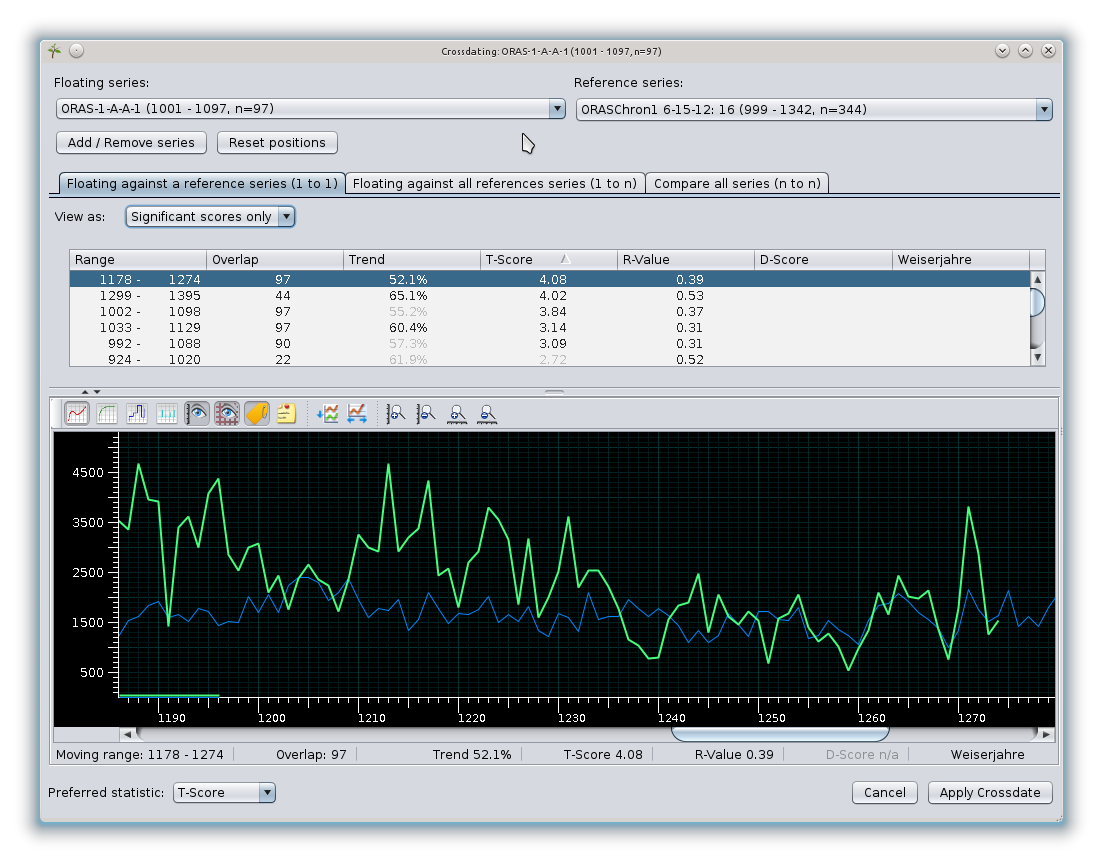
\includegraphics[width=\textwidth]{Images/crossdate1.png}
  \caption{Screenshot showing an example of the crossdating dialog.}
\end{figure}

At the top of the crossdate dialog it shows which series are currently being considered.  Top left is the floating series (the one that is of unknown date and is being moved to locate it's correct date position) and top right is the reference series (the series of known date).  If you loaded a pool of series you can uses these drop down menus to pick the series you want to compare.  You can also change the pool of series using button immediately below.  Below is a tabular and graphic representation of the crossdate that is being performed.  

Three tabs are provided for inspecting the statistical output of the various crossdating positions.  The first is a simple \textbf{1-to-1} comparison of the two series selected at the top of the screen.  This shows the various positions for the floating series against the reference chronology.   By selecting `Significant scores only' you will be presented with a simple table of the most statistically significant positions based upon your chosen statistical method, typically t-scores but other options can be chosen using the drop down menu at the bottom of the dialog.  By selecting rows in this table the graph below will update to shown the visual position of the crossdate selected.  Another option for exploring 1-to-1 crossdates is to view `All scores' which includes all positions whether they are significant or not.  Finally you can also choose `Histogram of scores' to explore the distribution of possible matches.

The next tab allows you to explore your floating series against all the other series in your pool (a \textbf{1-to-n} comparison).  This is useful for instance when you have an unknown sample that you are trying to match against a selection of reference chronologies e.g. as is typical in a dendroprovenancing study.  There are two options for the type of matches shown.  The first is a list of all the scores for the `floating' series in it's current chronological position against all the other series in the pool.  The second is a list of the best statistical match in any chronological position for the floating series against each of the series in the pool in turn.  The results of this analysis can be viewed either as a table or as a map.  In the latter, locations are shown for each of the series with the dot size relative to the statistical score.

The final tab shows the result of running all combination of series in the pool (a \textbf{n-to-n} comparison).  In this tab there is no distinction between floating and reference series.  Crossdates are run for each series against each of the other series and the details of the best match shown in the grid.  All series are treated as `floating' and no existing chronological positions are taken into consideration.  This method is largely reserved for a first-pass look when you have many samples of unknown date.  Clearly closer examination of potential matches must be done before proceeding.

At the bottom of the screen is a graphical representation of the current cross-match being examined.  The floating series on the graph is also click and draggable which means that manual visual cross-matches can be explored.  Below the graph the statistics for the current position are displayed.

Once you are satisfied you have a valid cross-match you can finish your crossdate by pressing the apply button.  This will create a new derived series based on your floating series but redated to the new chronological position.  You have the opportunity to explain your reasoning for choosing the cross-match and also give the match a broad star rating.  Once the newly dated series is committed, users can review the crossdate by viewing the history tab of the series, right clicking and selecting 'review crossdate'.  This provides a level of transparency that has not been possible before.  It's also a very useful tool for supervisors to assess the progress of students.


\section{Managing chronologies}
\index{Crossdating!Managing chronologies}
\index{Chronologies}

\index{Crossdating|)}
